\section{Task definition}

\begin{figure}
    \centering
    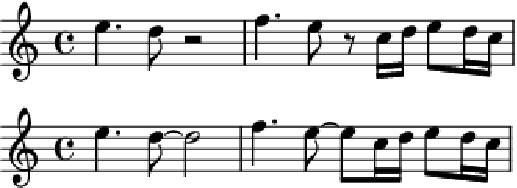
\includegraphics[width=8.1cm]{figs/heuristic_offsets.pdf}
    \caption{
The same note onsets engraved with ground truth~(top) vs. heuristic~(bottom) offsets. 
We argue that onset prediction suffices for producing melody transcriptions that are both recognizable and readable. 
}
 \label{fig:heuristic_offsets}
\end{figure}

% \john{You may want to lead here with two definitions: the definition of \emph{melody} (implicitly defined by labels) and the definition of \emph{melody transcription} (in contrast to melody extraction)}
% CHRIS: Added a footnote. Don't want to say too much more and risk getting lost in the weeds

We examine melody transcription, defined here as the task of converting music audio into a \emph{monophonic} (non-overlapping) sequence of \emph{notes} which constitute its melody.\footnote{Melody is tricky to precisely define---here we adopt an implicit definition based on crowdsourced melody annotations.} 
A note canonically consists of an onset time, a musical pitch, and an offset time, though in this work  
%(and as in~\cite{laaksonen2014automatic}) 
we disregard offsets for several reasons. 
First, accuracy of onsets has been found to be far more important to human perception of transcription quality than accuracy of offsets~\cite{ycart2020investigating}. 
Second, in our dataset (which constitutes a crowdsourced definition of melody), a heuristically-determined offset is identical to the ground truth offset for $89\%$ of notes.\footnote{The heuristic we adopt sets the offset of one note equal to the onset of the next, i.e., it assumes the melody is legato.}
Finally, we argue intuitively that onsets and pitches suffice for both recognizing and reading melodies---see~\Cref{fig:heuristic_offsets} for an example. 

Formally, a music waveform of length~$T$ seconds sampled at rate~$f_s$ is a vector~$\bm{a} \in \mathbb{R}^{Tf_s}$. The task of melody transcription is to convert $\bm{a}$ into a list of its melody notes~$\bm{y}$, where a note~$y_i$ is a pair of onset time~$t_i$ and musical pitch~$n_i$. Hence, 
\begin{gather*}
    %\bm{a} &= a_1, \ldots, a_S, \text{where}~S = Tf_s \\
    \bm{y} = y_1, \ldots, y_N, \\
    \text{where}~y_i = (t_i, n_i), t_i \leq T, \text{and}~n_i \in \{\text{A0}, \ldots, \text{C8}\}.
\end{gather*}
To handle the high dimensionality of audio, transcription algorithms typically extract features $\bm{X}$ (a matrix) from audio, which are sampled at $f_k \ll f_s$:
\begin{gather*}
    \text{Extract}(\bm{a}) = \bm{X} = \bm{x}_1, \ldots, \bm{x}_M, \\ 
    \text{where}~M = Tf_k, \text{and}~\bm{x}_i \in \mathbb{R}^d.
\end{gather*}
Hence, in practice, our goal is to build a transcription method 
% $f$ which maps features $\bm{X}$ to notes $\bm{y}$. 
$f : \bm{X} \mapsto \bm{y}$.

\subsection{Evaluation}
\label{sec:eval}

% CHRIS: This maps cleanly onto our contributions (standardized evaluation and new datasets), but may be too snarky for paragraph 2
%Finally, we argue that a historical focus on the important but disparate task of melody \emph{extraction}---detecting the time-varying fundamental frequency of the melody as opposed to its discrete notes---has led to a lack of work on transcription and systemic issues in evaluation.
% \john{Leading with an MIR implementation of F1 is a little confusing, especially since it is not typically applied to this task (you are defining the task, right?)}
% CHRIS: Reworked to clarify that this is a departure from melody extraction

To evaluate a melody transcription method $f$, 
we adopt a standard metric commonly used for evaluation in other music transcription tasks, namely,  ``onset-only notewise F-measure''~\cite{ycart2020investigating}. 
This metric scores an estimated transcript $f(\bm{X})$ by first matching its note onsets to those in the reference $\bm{y}$ with $50$ms of tolerance, and then computes a standard \fone{} score where an estimated note is treated as correct if it is the same pitch as its matched reference note. 
% \begin{equation*}
%      \text{\fone} : f(\bm{X}), y \mapsto [0, 1].
% \end{equation*}
This ``notewise'' metric represents a departure from the ``frame-based'' metrics typically used to evaluate melody extraction algorithms---Ycart~et~al.\ demonstrate in~\cite{ycart2020investigating} that this particular notewise metric correlates more strongly with human perception of transcription quality than any other common metric, including frame-based ones.

We make a small modification to this notewise metric to make it more appropriate for the melody transcription setting: an estimate $f(\bm{X})$ may receive full credit if it is off by a fixed octave shift but otherwise identical to the reference. 
In downstream settings, melody transcriptions are likely to be used in an octave-invariant fashion, e.g.,~they may be shifted to read more comfortably in treble clef, or performed by singers with different vocal ranges. 
Previous evaluations for melody extraction gave full credit for estimates with the right pitch class, ignoring octaves entirely (see~\cite{poliner2007melody} for a summary). 
However we argue that this is overly permissive, as \emph{relative} octave information preserves intervals between notes, and thus may be critical to the identity of a melody. 
Hence, we modify the evaluation criteria by simply taking the highest score over octave shifted versions of the estimate:
\begin{equation*}
    \max_{i \in \mathbb{Z}} \text{\fone}(\text{OctaveShift}(f(\bm{X}), i), \mathbf{y}).
\end{equation*}
Henceforth, we refer to this octave-invariant metric as \fone. 